\section {Исследовательский раздел}
В настоящем разделе будет произведён анализ различных возможностей исследования исполняемых (PE, Portable Executable) файлов, применяемых в настоящее время в различных средствах борьбы с вредоносным ПО, после чего  будут описаны некоторые из применяемых вирусами техник, присутствие которых в исполняемых образцах могло бы свидетельствовать об их подозрительном поведении. В идеале, нахождение и совмещение цепочек, реализующих такие техники в исследуемых образцах, и является целью предлагаемого к реализации программного модуля.

Также в разделе будут использованы фрагменты кода ассемблер под платформу x86 в синтаксисе Intel (операнд назначения указывается перед операндом, являющимся источником) в целях конкретизации описываемых техник.
\subsection {Исследование самоизменяющегося исполняемого кода}
В современном мире статический анализ исполняемых файлов играет важную роль в обнаружении вирусов. Однако, с момента первого использования этой техники прошёл не один десяток лет, и современные создатели вредоносного ПО способны использовать  различные методы, которые делают статический анализ неэффективным. Некоторые из таких техник заключаются в видоизменении исходного образца тем или иным образом и будут рассмотрены далее. 
\subsubsection {Полиморфизм}
Полиморфизм заключается в изменении случайным образом кода ПО так, чтобы сохранить изначальный функционал. Одним из простейших путей для реализации является шифрование участков кода, и расшифрование перед исполнением в памяти в определённый момент времени. Однако, это потребовало бы постоянного присутствия кода, реализующего расшифрование, и такой код мог бы являться в дальнейшем сигнатурой для данного вируса. В этом случае, приходится дополнительно использовать вспомогательные механизмы. Пусть у нас есть фрагмент кода, реализующий расшифрование. Как правило, такие участки кода достаточно просты и возможно произвольное изменение регистров, участвующих в таком коде, на другие, а также изменение порядка использования регистров. Фактически, такое действие изменяет последовательности байтов в файле, не меняя смысловой нагрузки программы. Далее, возможно где-либо хранить наборы допустимых замен регистров и во время исполнения программы случайным образом выбирать одну и использовать её. Однако, хранение наборов этих замен требует места, и возможно только для небольших участков кода, т.е. вся остальная часть программы должна быть зашифрована, при этом сам факт наличия зашифрованных участков кода может быть подозрительным (как правило, зашифрование исполняемого файла ведёт к появлению в нём невалидных или редко используемых машинных команд).
\subsubsection {Метаморфизм}
Метаморфизм является следующим логическим шагом после техники полиморфизма. Вместо того, чтобы шифровать всю программу целиком и менять процедуру расшифрования, следует создавать различные версии программы каждый раз, когда она вновь исполняется. Это требует встраивания в тело программы процедуры, которая проводила бы анализ кода программы и изменение её на лету. Причём, такие изменения выполняются не только над самой программой, но и над анализирующей её процедурой. Ключевым моментом здесь является набор изменений, который может реализован данной процедурой:
\lstset{style=masm}

\begin {itemize}
	\item Выбор используемых инструкций и регистров - например, для обнуления регистра eax могут быть использованы каждая из следующих семантически эквивалентных инструкций:
	\begin{lstlisting}
	mov eax, 0
	xor eax, eax
	sub eax, eax
	\end{lstlisting}
	\item Выбор порядка использования инструкций - в некоторых случаях допустимо, если инструкции независимы. Например, иногда современные компиляторы для оптимизации выполнения кода на современных процессорах, использующих конвейеризацию, откладывают выполнение условных переходов для создания возможности параллельного исполнения. Рассмотрим следующий участок кода:
	\begin{lstlisting}
	mov     cl, [edx+eax];
	add     bl, cl
	inc     eax
	cmp     eax, ebp; <-
	mov     [esi], bl;
	jb      short loc_401236; <-
	\end{lstlisting}
	Указанные стрелочкой инструкции логически должны бы следовать друг за другом, однако между ними была добавлена дополнительная инструкция, которая могла бы идти перед сравнением или после выполнения условного перехода. Перемещение её в указанное стрелочкой место, например:
	\begin{lstlisting}
	mov cl, [edx+eax]
	add bl, cl
	inc eax
	mov [esi], bl; <-
	cmp eax, ebp
	jb short loc_401236
	\end{lstlisting}
незначительным образом сказывается на производительности кода, однако, для вредоносного ПО большее значение имеет происходящее при этом изменение порядка байтов, влиящее на сигнатуру
	\item Обращение условных переходов. Многие современные компиляторы всё ещё используют генерацию условных переходов, соответствующую статическому алгоритму предсказания переходов процессоров семейства Intel NetBurst (Pentium 4 и др.)\cite{INTELMANUAL}. Алгоритм заключается в предсказании условного перехода на инструкции, следовавшие ранее (помогает для циклов) и предсказании отсутствия перехода на инструкции, следующие далее (помогает для конструкций if /else в том случае, когда в среднем чаще выполняется блок, следующий непосредственно после if). Аналогично компиляторам, метаморфические вирусы могут обнаруживать блоки таких условных конструкций и переставлять их местами в коде программы, когда такое возможно.

Пример:
	\begin{lstlisting}
	call    lstrcmpA
	jnz     short loc_4012D4
	push    40h; 1
	push    offset aCaption; 1
	push    offset aRightAnswer; 1
	push    [ebp+hWnd]; 1
	call    MessageBoxA; 1
	jmp     short loc_4012E8
loc_4012D4:
	push    10h; 2
	push    offset aCaption; 2
	push    offset aWrongAnswer; 2
	push    [ebp+hWnd]; 2
	call    MessageBoxA; 2
loc_4012E8:
	call    ExitProcess
	\end{lstlisting}
	Замена первоначальной инструкции jnz на jz (переход в случае неравенства на переход в случае равенства) и перестановка местами блоков, помеченных как 1 и 2 не меняет смысловую нагрузку, выполняемую программой, однако позволяет значительно поменять её структуру. Это создаёт значительные трудности как в случае автоматического, так и ручного исследования, если таковых замен произведено значительное количество.
	\item Добавление мусора - заключается в произвольном добавлении инструкций, не влиящих на ход исполнения самой программы. Например, манипуляции с регистром, не используемым в определённом фрагменте кода:
	\begin{lstlisting}
	mov     bl, [edi+ecx]
	lea     esi, [edi+ecx]
	add     ebx, eax <-
	add     ebx, esi <-
	add     ebx, ecx <-
	mov     cl, [edx+eax]
	add     bl, cl
	inc     eax
	xor     ebx, ebx
	\end{lstlisting}
	Указанные стрелочкой инструкции никак не влияют на программу в случае их добавления, поскольку далее ebx всё равно обнуляется.
	\item Изменение порядка хранения функций в модуле - не сказывается на функционале, однако точно так же меняет байтовые сигнатуры, а также может вводить в заблужение лиц, выполняющих ручной анализ.
\end {itemize}

\subsection{Изучение возможностей динамического анализа}
Полиморфические вирусы поддаются обнаружению на основе статистического анализа \cite{PAYLOADDETECTION, ANAGRAM}, используя распределение частот редко появляющихся байтов, а также на основе анализа энтропии различных секций файла \cite{ENTROPYANALYSIS}. Метаморфические могут быть распознаны различными техниками семантического анализа графа потока исполнения, построенного на основе обнаруживаемых в исходном файле инструкций вызова функций \cite{METAAWARE}. Однако, для борьбы со всеми вышеупомянутыми методами обнаружения была предложена новая техника маскирования кода вредоносных программ - мимиморфизм\cite{MIMIMORPHISM}. Описание механизма реализации данной техники выходит за рамки данного проекта, однако, достаточно сказать, что в результате её работы получаются исполняемые файлы, статистические характеристики, а также граф исполнения которых похожи на обычное ПО. Таким образом, каждая из упомянутых статических техник анализа рано или поздно достигает своих пределов.

В связи с этим, выглядит неизбежным применение динамического анализа исполняемых файлов. В последнее время большое распространение получили ``песочницы'' --- изолированные среды, в рамках которых выполняются исследуемые образцы и происходит сбор изменений, вызванных их деятельностью (Cuckoo Sandbox, используемый в проекте VirusTotal, а также Sandboxie, Nepenthes, Dionaea и др.). Многие из них основываются на поиске особых ``артефактов'' --- изменений в файловой системе, реестре, директории именованных объектов (BaseNamedObjects, там находятся все мутэксы --- объекты синхронизации, обычно используемые для проверки факта заражённости ПК, чтобы не дать исполняться одновременно многим копиям вируса), списке открытых хэндлов у системных (и не только) процессов и многих других. Однако, согласно последним прогнозам рынка производителей антивирусных программ\cite{KASPERKSYBULLETIN}, всё большее число вирусов будет стараться отходить от принципа Advanced Persistent Threat (APT). Факт постоянного присутствия (Persistent) после заражения уйдёт в сторону находящихся лишь в памяти вирусов (без файлов), чтобы максимально уменьшить число следов, оставляемых после заражения с целью избежания обнаружения. Факт ``продвинутости'' (Advanced) вирусов, использующих неординарные подходы (в прошлом году прошла волна вируса Carbanak\cite{CARBANAK}, который для реализации механизма скрытия модифицировал прошивку жёстких дисков) и требующих больших затрат на разработку уйдёт в сторону переиспользования уже существующих и появляющихся популярных семейств. Самым естественным для анализа при этом выглядит использование одной из существенных черт любой программы - её взаимодействие с ОС непосредственно в процессе работы через вызовы API функций, причём существенная часть этих вызовов по сути неизбежна. Поэтому, представляется важным нахождение ``отпечатка'' тех или иных фрагментов поведения программы.

\subsection {Рассмотрение способов отслеживания происходящих событий}
Для реализации анализатора поведения программ необходимо обеспечить качественный сбор информации о происходящих во время исполнения событиях. Далее будут рассмотрены доступные способы реализации такого анализа и выбран наиболее подходящий из них в рамках данной работы.
Для решения указанной проблемы нужно найти способ получения происходящих в исполняемых процессах событий. 

Мониторинг API, пути решения:
\begin {itemize}
	\item Перехватывающая вызовы API DLL (пр.: Microsoft Detours);

	В том числе : AppInit\_DLL – но лишь в том случае, если приложение использует user32.dll.
	\item Перехватывающий вызовы API драйвер (пр.: Process Hacker).
	\item Отслеживание вызовов в отладчике, пример реализации дан в \cite{MALWAREBOOK}.
	\item Процедуры, выполняющие уведомления о создании процесса/ потока/ загрузке образа в память (пр.:
 	ProcMon, Process и Thread events).
\end {itemize}

\subsubsection {Перехватывающая вызовы API DLL}
Рассмотрим подробнее данный способ. Если мы хотим перехватить вызовы N функций в текущем процессе,
 в его адресное пространство после загрузки системных библиотек, содержащих функции, которые необходимо
 отслеживать, мы загружаем нашу cпециально сформированную DLL библиотеку. В своей входной функции,
 выполняющейся во время загрузки, она перезаписывает адреса в таблице импортов процесса на адреса своих
 функций, в которых выполняется логирование вызова, после чего вызывается оригинальная функция. Таким образом, если требуются различные действия для каждой отслеживаемой функции, в нашей DLL будет отдельно
 содержаться функция для каждой из N.
 
В Windows существует специальный раздел реестра, с помощью которого можно загрузить данную DLL в память. AppInit\_DLL - раздел реестра, в который можно поместить пути до всех DLL, которые будут загружены в адресное пространство исполняемых в текущем сеансе процессов при их инициализации. Однако, это сработает только в том случае, когда исполняемый файл содержит импорты из user32.dll, так что полагаться на этот способ возможно не всегда.
\subsubsection {Перехватывающий вызовы API драйвер}
 Концепция аналогична перехватывающей вызовы API DLL, однако адреса в данном случае перезаписываются не в таблице импортов исследуемого процесса, а SSDT (System Service Descriptor Table), что изначально требует найти начало этой таблицы в памяти. SSDT (Native SSDT) - служебная таблица в Windows, хранящая указатель на таблицу с адресами функций, реализующих те или иные системные вызовы. Когда любой программе требуется реализовать системный вызов, она берёт порядковый номер функции в этой таблице и вызывает инструкцию процессора SYSENTER.  При данном вызове системная служебная функция KiSystemService забирает этот порядковый номер, смотрит в SSDT и выбирает функцию, индекс которой соответствует переданному в младшей части регистра eax числу.

Напрямую из режима пользователя получить адрес Native SSDT нельзя. Это обычно делается вызовом MmGetSystemRoutineAddress, что возможно только в режиме ядра. Для этого загружается драйвер, выполняющий указанные действия.
\subsubsection {Перехват вызовов в отладчике}
Для реализации данного функционала в отладчике достаточно установить точки останова (байт 0xCC, соответствующий инструкции программного прерывания int 0x3) на старший байт первой инструкции каждой библиотечной функции, вызов которой необходимо отслеживать. При срабатывании прерывания операционная система передаёт управление отладчику, если он подключён к процессу, в котором оно произошло. Дальнейшая необходимая обработка выполняется в самом отладчике, после чего он подаёт команду на продолжение исполнения процесса.
\subsubsection {Процедуры уведомления}
В Windows существует набор процедур уведомления, таких, как PsSetCreateProcessNotifyRoutine, PsSetCreateThreadNotifyRoutine и др., которые могут отправлять уведомления в случае возникновения указанных событий (таких, как создание или завершение процесса или потока). Для этого драйвер, который хочет получать уведомления, должен зарегистрироваться на них, вызвав соответствующую функцию и передав указатель на самостоятельно реализумый обработчик . Однако, в данном случае полная полученная информация состоит лишь из pid процесса и флага, указывающего факт создания или завершения. Примером реализации такого подхода может служить утилита ProcessMon из набора SysInternals от Марка Руссиновича.
\subsection {Выбор реализуемого способа динамического анализа}
Одновременно наиболее простой и захватывающей наибольший возможный контекст вызовов реализацией представляется перехват событий через отладчик.

Существует множество бесплатного ПО, реализующего функционал отладчиков. Наиболее примечательным из них для исследования вирусов можно считать Immunity Debugger, изначально проектировавшийся как инструмент для разработки эксплоитов, реверсинга исполняемых файлов и анализа вредоносного ПО. Некоторые из его преимуществ по сравнению с обычными отладчиками:
\begin {itemize}
	\item Изначально Immunity разрабатывался на основе старого популярного отладчика - OllyDbg, одним из преимуществ которого была поддержка плагинов. Однако, плагины для OllyDbg представляли собой динамические библиотеки (DLL), требующие компиляции перед использованием. Плагины для Immunity представляют собой скрипты Python, которые можно изменять в любом текстовом редакторе и использовать сразу же.
	\paragraph {PyCommands}
Immunity Debugger поддерживает реализацию определённой последовательности действий, описанную в скрипте на ЯП Python - PyCommand, которая может быть вызвана через его консоль. Также PyCommand поддерживают хуки - описанные функции, которые будут вызваны в случае возникновения настроенного на них события (обычно, срабатывание прерывания отладки в установленной точке останова).
	\item Immunity содержит в комплекте множество готовых плагинов. Один из них реализует некоторые техники по скрытию факта присутствия отладчика (!hidedebug). Его функционал будет использован в цикле исследования вредоносных образцов. Также, сообществом Python уже созданы реализации многих популярных задач, например, сбор всех функций из таблицы импортов исполняемого файла (mona.py от Corelan GCV). Данный функционал используется для реализации собственного хука, логирующего необходимые данные.
	\item В Immunity реализован механизм автоматического обнаружения упакованных исполняемых файлов. Также есть функционал, позволяющий обнаружить оригинальную точку входа такого исполняемого файла, если используемый в данном файле упаковщик применял тривиальный алгоритм. Дело в том, что в таблице импортов упакованного файла находятся лишь те функции, которые необходимы для процедуры распаковки, а записи о функциях, требуемых для работы оригинального исполняемого файла добавляются в течение распаковки. Если установить отслеживание только первоначально присутствующих функций, большая часть информативности логов будет утеряна.
\end {itemize}

Поскольку Immunity работает только с x86, исследуемые образцы следует предварительно фильтровать по значению платформы, хранящемуся в PE-заголовке исполняемого файла.
\subsection {Примеры последовательностей, используемых вредоносным ПО}
\subsubsection {Backdoor.Hacarmy.D}
Пример разбора функционирования одного из современных вирусов, использующего сетевые соединения для
получения команд от управляющего узла дан в \cite{REVERSING}. Для инфицирования там используется следующая последовательность вызовов API функций:
\begin {enumerate}
	\item kernel32.GetModuleFileNameA
	\item kernel32.GetSystemDirectoryA
	\item user32.CharUpperBuffA
	\item crtdll.strstr
	\item crtdll.strcat
	\item kernel32.Sleep
	\item kernel32.CopyFileA
	\item kernel32.ShellExecuteA
	\item kernel32.ExitProcess
\end {enumerate}
После инфицирования вирус заново исполняет себя, но при этом уже из системной директории, удаляя оригинальный исполняемый файл. При этом для избежания многократного заражения используется объект синхронизации, обладающий уникальным именем - мутэкс.
\begin {enumerate}
	\item kernel32.DeleteFileA
	\item kernel32.CreateMutexA
	\item kernel32.GetLastError
\end {enumerate}
В случае, если данный именованный объект синхронизации уже присутствует в системе --- при вызове CreateMutex происходит ошибка, GetLastError возвращает её код и программа завершает работу. Если всё прошло успешно, для получения управляющих команд начинается главная часть программы - бесконечный цикл, в котором проверяется валидность IP адреса ПК, а в случае провала - ожидание (wininet.InternetGetConnectedState -> kernel32.Sleep), после чего получаются и исполняются соответствующие удалённые команды.
\subsubsection {Техника полого процесса}
Вирусы, использующие для работы собственные процессы, могут быть обнаружены по расположению их файлов исполняемых образов на жёстком диске, даже если они используют те же имена, что и у системных процессов. Однако, существует техника маскирования \cite{MALWAREBOOK}, при которой даже путь расположения будет совпадать с легитимными системными файлами.
Рассмотрим следующую последовательность вызовов:
\begin {enumerate}
	\item CreateProcessA (..., CREATE\_SUSPENDED, ...)
	\item ReadFile
	\item GetModuleHandleA
	\item GetProcAddress
	\item NtUnmapViewOfSection
	\item VirtualAllocEx (..., PAGE\_EXECUTE\_READWRITE, ...)
	\item WriteProcessMemory (в цикле)
	\item SetThreadContext
	\item ResumeThread
\end{enumerate}
По сути, она просто запускает какой-либо системный процесс в приостановленном состоянии, удаляет часть страниц его памяти начиная с базового адреса вируса, который будет скопирован в чужое адресное пространство, выделяет для себя новую память (поскольку обычно страницы, хранящие секцию кода не имеют атрибута, разрешающего запись) и после этого продолжает исполнение изначально остановленного потока, установив нужный контекст потока, и наконец указатель инструкций на оригинальную точку входа (Original Entry Point, OEP) в тело вируса. Для легитимного использования таких действий не представляется возможным найти каких-либо причин, поэтому можно считать, что такая последовательность свидетельствует о вредоносности исполняемого файла.

\subsection {Рассмотрение потенциально подозрительных обращений к ОС через библиотечные функции}
В различных версиях Windows существует множество динамических библиотек. К базовым обычно относят:
\begin {itemize}
	\item ntdll.dll --- экспортирует так называемые ''родные`` (англ. Native API) функции ядра (набор функций, реализуемых ядром операционной системы - обычно ntoskrnl.exe);
	\item kernel32.dll --- экспортирует функции, отвечающие за управление памятью, вводом-выводом, управление процессами/потоками, однако является в основном лишь ''обёрткой`` над родными API функциями из ntdll.dll;
	\item user32.dll --- высокоуровневую библиотеку для управления графическим интерфейсом;
	\item gdi32.dll --- низкоуровневую библиотеку рисования.
\end {itemize}
Также в контексте работы вредоносного ПО важное значение имеют такие библиотеки, как sfc\_os.dll - отвечает за Windows File Protection (функцию защиты от перезаписи важных системных файлов), pstorec.dll - реализует доступ к управляемому Windows защищённому хранилищу паролей.

Большая часть интересующих нас функций, которые будут использовать исследуемые образцы, находится  обычно в kernel32, однако возможно и прямое импортирование  из ntdll. Тем не менее, ситуации, когда такое может происходить, довольно специфичны --- например, легальное применение Native API обычно присутствует только в антивирусных продуктах.
В процессе запуска исполняемых файлов одним из значимых событий является создание новых процессов, особенно в случае слежения за образцами с помощью отладчика, т.к. все действия, происходящие в новом процессе, не будут отслежены без специальных дополнительных действий. Также большое значение в действиях вредоносного ПО имеет манипуляция файлами на инфицированном ПК, например, удаление. Далее будут описаны в качестве примера механизмы удаления файла и создания процесса в Windows.

\subparagraph {Удаление файлов}
Как мы можем видеть на рисунке \ref{fig:filedelete}, у пользовательских программ есть два основных пути
для удаления файлов:
\begin {figure}[h]
	\centering
	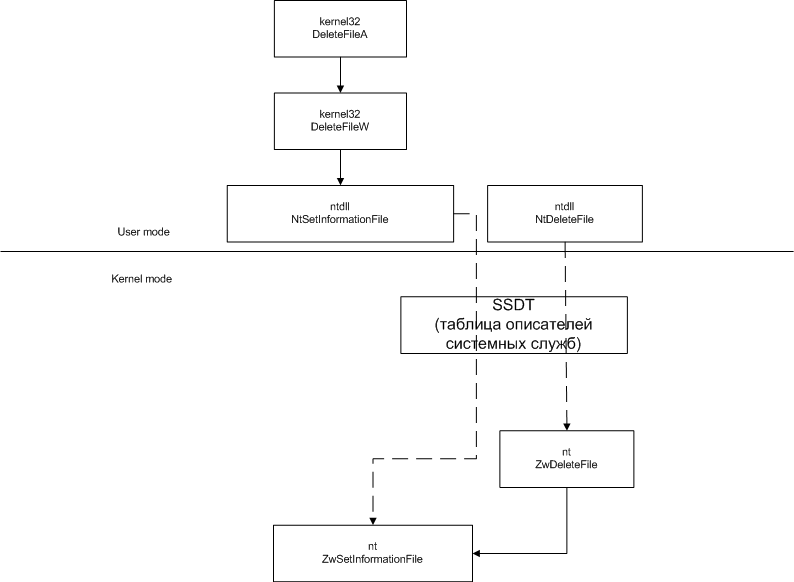
\includegraphics[width=\linewidth]{img/DeleteFileAPIs.png}
	\caption{Функции, отвечающие за удаление файлов}
	\label{fig:filedelete}
\end {figure}
На схеме изображена последовательность вызывающих друг друга функций для реализации удаления. Из неё следует, что в результате запроса об удалении файла ОС всего лишь помечает атрибуты объекта файла на удаление, а само удаление выполняется другим механизмом. Однако, существуют и другие способы удаления файлов. Например, если файл был создан функцией CreateFile с флагом FILE\_FLAG\_DELETE\_ON\_CLOSE, он будет удалён после закрытия все хэндлов и удаления всех ссылок на него без дополнительных обращений из режима пользователя (это пример техники, используемой вирусами для уничтожения следов после осуществеления вредоносной деятельности в системе).
\subparagraph {Создание процессов}
Для создания процессов есть множество различных путей, в том числе, и за рамками приведённых API функций, и нельзя полагаться, что любой создаваемый процесс будет обнаружен, если следить только за ними (рисунок  \ref{fig:createprocess}).
\begin {figure}[h]
	\centering
	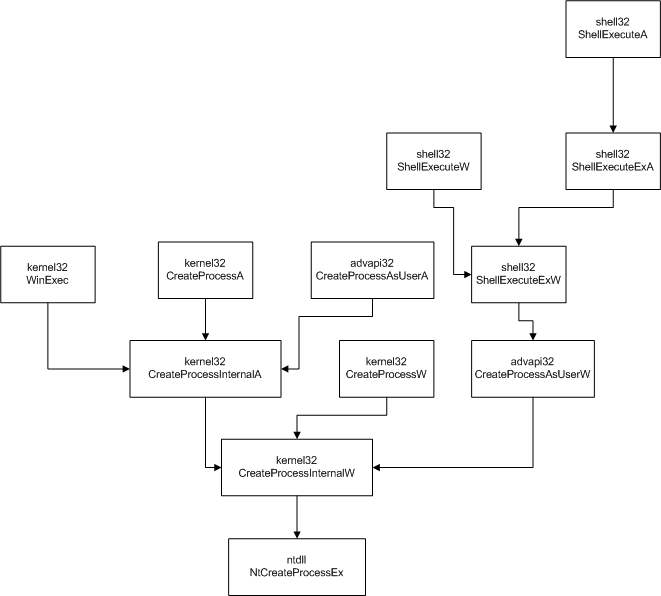
\includegraphics[width=\linewidth]{img/ExampleProcessCreateAPIs.png}
	\caption{Функции, отвечающие за создание процесса}
	\label{fig:createprocess}
\end {figure}
\subsection {Выводы по разделу}
В настоящем разделе был произведён анализ ограничений статических методов исследования исполняемого кода, рассмотрены возможные методы реализации динамического анализа, выбран имеющий наибольшие преимущества и являющийся достаточно простым в реализации вариант, а также проанализированы группы некоторых из Windows API функций, использование которых представляется наиболее значительным при рассмотрении поведения программных средств на наличие подозрительных признаков.